\documentclass[a4paper, 12pt]{article}
% Allows writing the document in French.
\usepackage[T1]{fontenc}
\usepackage[utf8]{inputenc}
\usepackage[francais]{babel}
% Allows to change the margins of the pages.
\usepackage[margin=2.5cm]{geometry}
% Allows to change the line spacing.
\renewcommand{\baselinestretch}{1.5}
% Provides generic commands \degree, \celsius, etc.
\usepackage{gensymb}
% Allows to use images.
\usepackage{graphicx}
% Includes pseudocode or algorithms.
\usepackage{listings, lstautogobble}
% Allows change items properties
\usepackage{enumitem}
% Adds space between paragraphs.
\usepackage{parskip}
% Supports Text Companion fonts (necessary for gensymb).
\usepackage{textcomp}
% Allows to create better tables.
\usepackage{tabularx}
% Allows to draw.
\usepackage{tikz}
% Allows to color the raw of an array.
\usepackage{colortbl}
% Allows to use colors.
\usepackage{xcolor}
% Allows hyperlinks within the document.
\usepackage[colorlinks=true,urlcolor=black,linkcolor=black]{hyperref}
% Allows to use copyright.
\usepackage[
    type={CC},
    modifier={by-nc-nd},
    version={4.0},
    ]{doclicense}

% Allows a better depth for the table of contents.
\setcounter{tocdepth}{2}
% Allows a better depth for the sections.
\setcounter{secnumdepth}{4}

% New column type
\newcolumntype{L}{>{\raggedright\arraybackslash}X}
\newcolumntype{C}{>{\centering\arraybackslash}X}
\newcolumntype{R}{>{\raggedleft\arraybackslash}X}

% Define colors for color scheme
\definecolor{black}{HTML}{333333}
\definecolor{currentLine}{HTML}{282A2E}
\definecolor{selection}{HTML}{373B41}
\definecolor{grey}{HTML}{EEEEEE}
\definecolor{comment}{HTML}{969896}
\definecolor{red}{HTML}{CC6666}
\definecolor{orange}{HTML}{DE935F}
\definecolor{yellow}{HTML}{F0C674}
\definecolor{green}{HTML}{B5BD68}
\definecolor{aqua}{HTML}{8ABEB7}
\definecolor{blue}{HTML}{81A2bE}
\definecolor{purple}{HTML}{B294BB}
\definecolor{bleuSkype}{HTML}{00AFF0}
\definecolor{jauneSnapchat}{HTML}{FFFC00}

% Macro
\makeatletter
\lst@InstallKeywords k{attributes}{attributestyle}\slshape{attributestyle}{}ld
\makeatother

% Custom color scheme for bash.
\lstset{language=bash,
  basicstyle=\ttfamily\color{black},
  numbers=left,
  stepnumber=1,
  numberstyle=\tiny,
  autogobble=true,
  backgroundcolor=\color{grey},
  commentstyle=\color{comment},
  stringstyle=\color{green},
  keywordstyle=\color{red},
  keywords={home, root, user, @, \$},
  attributestyle=\color{aqua},
  moreattributes={ls, now}
}

% Allows draw lines for the flyleaf.
\newcommand{\HRule}{\rule{\linewidth}{0.5mm}}

% Starts roman numbering (trick to not numbering the first pages).
\pagenumbering{roman}

\begin{document}
\renewcommand{\bibname}{Références}
\begin{center}
  
\includegraphics[scale=0.12]{textures/logo/heh_bw.pdf}

  \vspace{1cm}

  \textsc{\LARGE Projet} \\ [0.5cm]
  \textsc{\Large Réalisation d'un site en PHP} \\ [0.5cm]

  \textsc{\large 2\up{ème} Bachelier en Informatique} \\ [0.2cm]

  \begingroup
  \fontfamily{pag} \selectfont 

  \HRule \\ [0.4cm] {
    \huge Programmation web \\ [0.2cm] 
  }
  \HRule \\ [1.3cm]
  \endgroup
  \begin{minipage}[t]{0.4 \textwidth} 
    \begin{flushleft} 
      \large \emph{Auteur:} \\ 
      Alexandre \textsc{Ducobu}
    \end{flushleft} 
  \end{minipage}
  % 
  \begin{minipage}[t]{0.4 \textwidth}
    \begin{flushright} 
      \large \emph{Enseignants :} \\ 
      Antoine \textsc{Malaise} \\
      Fabrice \textsc{Scopel}
    \end{flushright} 
  \end{minipage}

  \vspace{1cm}

  
\includegraphics[scale=0.08]{textures/logo/technical_bw.pdf}

  \vspace{0.5cm}

  Année académique 2016 - 2017
\end{center}

\thispagestyle{empty}

\newpage
\newpage
\thispagestyle{empty}
\setcounter{page}{0}
\null
\newpage
\begin{center}
  
\includegraphics[scale=0.12]{textures/logo/heh.pdf}

  \vspace{2cm}

  \textsc{\LARGE Projet ARS} \\ [0.5cm]
  \textsc{\Large Les différents systèmes d'exploitation} \\ [0.5cm]

  \textsc{\large 1er Bachelier en Informatique} \\ [0.2cm]
  \textsc{Groupe 5-8} \\

  \begingroup
  \fontfamily{pag} \selectfont 

  \HRule \\ [0.4cm] {
    \huge Architecture des Systèmes II \\ [0.2cm] 
  }
  (Laboratoire)
  \HRule \\ [1.3cm]
  \endgroup

  \begin{minipage}[t]{0.4 \textwidth} 
    \begin{flushleft} 
      \large \emph{Auteur:} \\ 
      Agozzino \textsc{Terencio} 
    \end{flushleft} 
  \end{minipage}
  % 
  \begin{minipage}[t]{0.4 \textwidth}
    \begin{flushright} 
      \large \emph{Auteur :} \\ 
      Ducobu \textsc{Alexandre} 
    \end{flushright} 
  \end{minipage}

  \vspace{0.5cm}

  \begin{minipage}[t]{0.4 \textwidth}
    \begin{center} 
      \large \emph{Enseignant:} \\ 
      Desmet \textsc{Erwin} 
    \end{center} 
  \end{minipage}

  \vspace{0.5cm}

  
\includegraphics[scale=0.08]{textures/logo/technical.pdf}

  \vspace{0.5cm}

  Année académique 2015 - 2016
\end{center}

\thispagestyle{empty}

\newpage
\newpage
\thispagestyle{empty}
\setcounter{page}{0}
\null
\newpage
\newpage
\mbox{~}
\vfill
Ce document est mis à disposition selon les termes de la licence Creative
Commons ``\href{https://creativecommons.org/licenses/by-nc-nd/4.0/}{Attribution -
Pas d'utilisation commerciale 4.0 International}''.

\begin{figure}[!h]
  \centering
  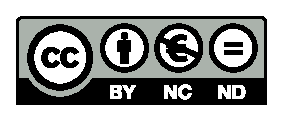
\includegraphics[width=0.25\textwidth]
  {textures/images/license/license.eps}
\end{figure}

\thispagestyle{empty}

\newpage
\pagenumbering{arabic}
\tableofcontents
\newpage
\section{Présentation générale du projet}
\label{sec:pres-gener-du}

\subsection{Introduction}
\label{subsec:introduction}

Dans le cadre de ce projet, il nous a été demandé d'administrer un serveur sous
Linux.

Le choix de la distribution ainsi que la gestion des sauvegardes est libre et
devra être justifié.

Le serveur devra contenir :
\begin{itemize}
\item un partage NFS qui permettra aux utilisateurs du réseaux local d'y stocker
des fichiers ;

\item un partage Samba qui permettra aux utilisateurs de Windows d'accéder à ce
même partage ;

\item un serveur Web, FTP, MySQL et DNS qui permettra un hébergement
multi-utilisateurs ;
  \begin{itemize}
  \item[\tiny$\bullet$] le serveur FTP permettra à chaque utilisateur d'accéder
à son dossier Web ;
  \item[\tiny$\bullet$] le serveur DNS contiendra une zone qui sera
    indispensable pour les sites Web de l'utilisateur ;

  \item[\tiny$\bullet$] le serveur DNS fera également office de DNS cache pour
le réseau local.
  \end{itemize}

\item un serveur NTP pour que les machines du réseau local puissent se
synchroniser ;

\item le support du module SSH.
\end{itemize}

\newpage

\subsection{Déontologie}
\label{subsec:déontologie}

En tant qu'administrateurs du serveur, nous serons tenus de suivre de nombreuses
règles telles que :
\begin{itemize}
\item la documentation des actions entreprises sur le serveur;
\item l'automatisation des installations et configurations au travers de scripts;
\item la sécurité : mise en place de mots de passe forts, du SSH, etc. ;
\item la vigilance et la prévoyance, par exemple par la mise en place de
  sauvegardes avant et après chaque changement sur le serveur ;
\item le contrôle du bon fonctionnement de chaque élément.
\end{itemize}

\subsection{Sécurité}
\label{subsec:securite}

Du côté de la sécurité, quelques contraintes seront prises en compte :
\begin{itemize}
\item mise en place d'une politique utilisateur ;
\item mise en place de quotas ;
\item partitionnement et gestion du disque (LVM et RAID) ;
\item mise en place d'une stratégie de sauvegarde ;
\item désactivation des éléments inutiles et des mises à jours ;
\item mise en place d'un antivirus, d'un firewall, etc.
\end{itemize}

%%% Local Variables:
%%% mode: latex
%%% TeX-master: t
%%% End:

\newpage
\section{Choix}
\label{sec:choix}

\subsection{Langage}
\label{sec:langage}

Pour ce projet, notre choix s'est naturellement porté vers le Python.
En effet, en plus d'être le langage de prédilection sur le Raspberry Pi, il dispose d'une
documentation et d'une vaste communauté. \\
En outre, ce langage apporte une facilité pour l'interaction avec les
GPIO \footnote{General-purpose input/output} de la Raspberry Pi et la librairie du
Sense HAT.

\subsection{Raspbian}
\label{sec:raspbian}

Pour notre utilisation, Raspbian, étant le choix suggéré par le constructeur, a été choisi.

\begin{figure}[!h]
  \centering
  
\includegraphics[scale=0.06]
  {textures/images/choices/raspbian.pdf}
  \caption{Logo Raspbian}
  \label{fig:raspbian}
\end{figure}

\subsection{Outils de développement}
\label{sec:outils-de-devel}

GNU Emacs et Atom ont été les seuls éditeurs de texte utilisés comme outils de
développement pour leur simplicité ainsi que pour notre familiarité avec ceux-ci.

\begin{figure}[!h]
\centering
\begin{minipage}[c]{0.4\textwidth}
  \centering
  
\includegraphics[scale=0.09]
  {textures/images/choices/emacs.pdf}
\caption{Logo Emacs}\label{emacs}
\end{minipage} \qquad
\begin{minipage}[c]{0.4\textwidth}
  \centering
  
\includegraphics[scale=0.09]
  {textures/images/choices/atom.pdf}
\caption{Logo Atom}\label{atom}
\end{minipage}
\end{figure}

De plus, nous avons utilisé GitHub qui est un service en ligne permettant
d'héberger notre projet et de ce fait, synchroniser notre travail.

\begin{figure}[!h]
  \centering
  
\includegraphics[scale=0.1]
  {textures/images/choices/github.pdf}
  \caption{Logo GitHub}
  \label{fig:github}
\end{figure}

%%% Local Variables:
%%% mode: latex
%%% TeX-master: t
%%% End:
\newpage
\section{Services}
\label{sec:services}


\section{Base de données}
\label{sec:BD}


\subsection{Création de la base de données}
\label{sec:creation-db}

La base de données est composée de trois tables contenant toutes les données utiles au bon fonctionnement du site.\\
Il y a la table \textbf{Users} \textit{pour tout ce qui concerne les utilisateurs}, la table \textbf{Medicines}, \textit{qui concerne les médicaments} et le table \textbf{Reserves} \textit{qui contient la réserve de chaque utilisateur}.

\begin{figure}[h]
  \centering
  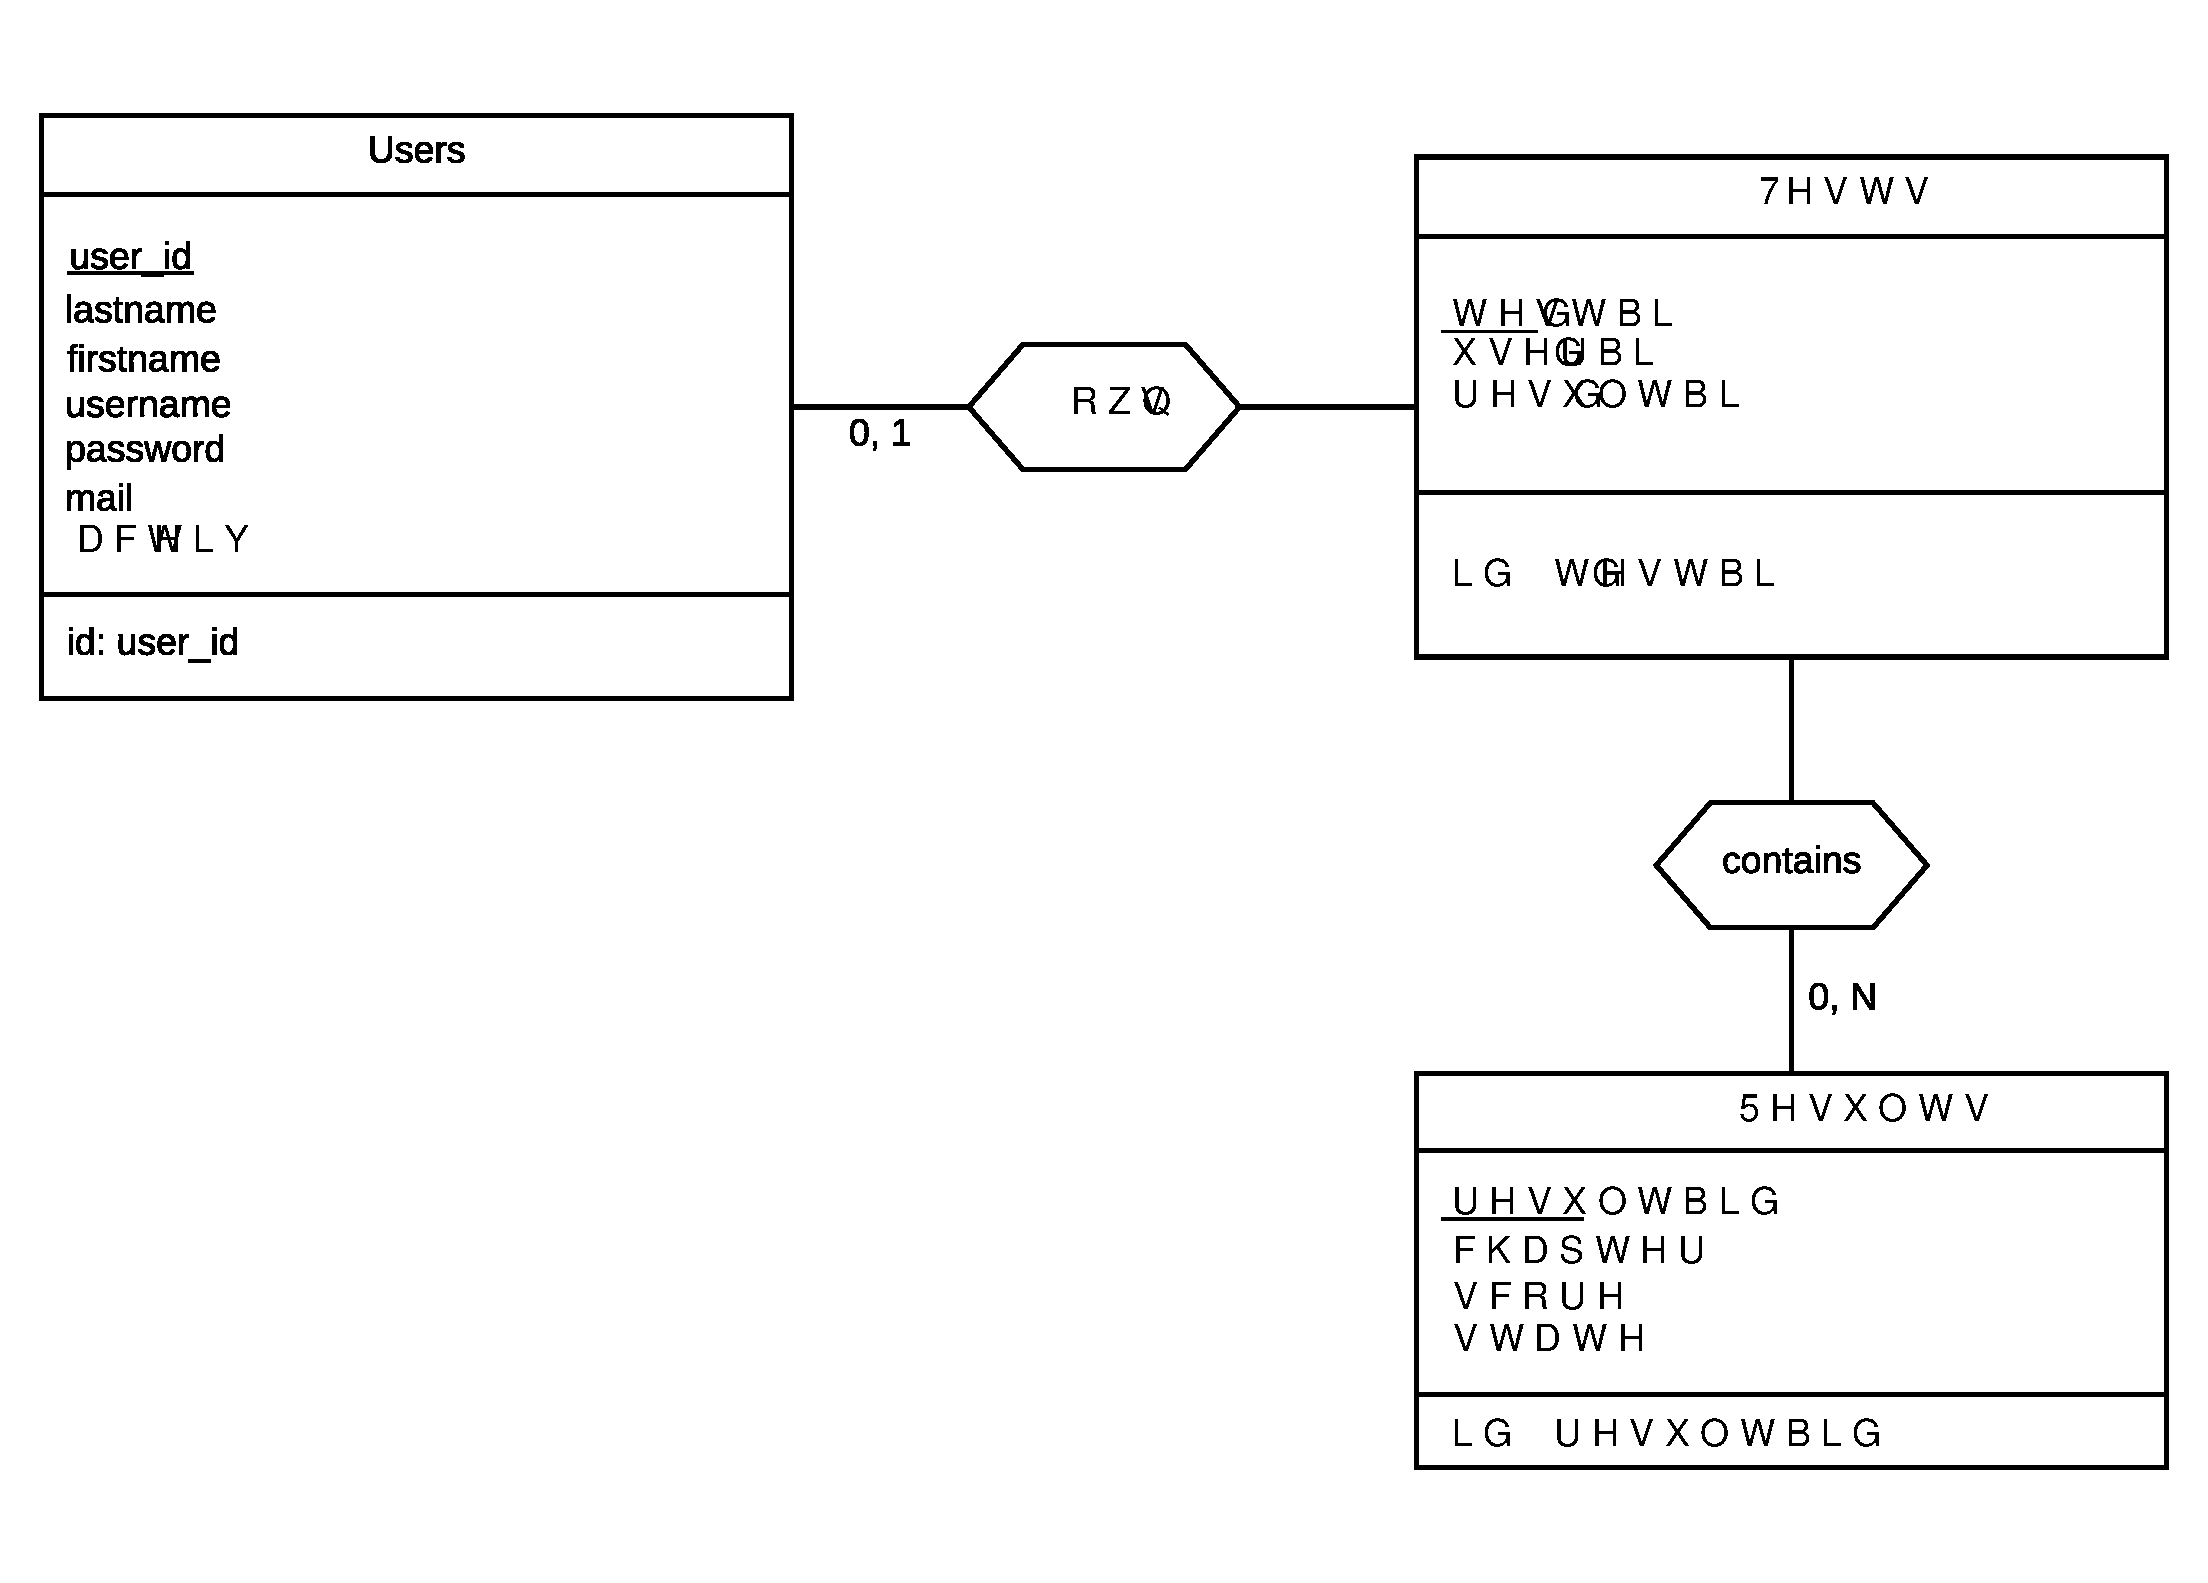
\includegraphics[scale=0.4]
  {textures/images/db/DB.pdf}
  \caption{Schéma conceptuel de la base de données}
  \label{fig:db}
\end{figure}

\newpage

\subsection{Vue détaillée}
\label{sec:vue-details}


\subsubsection{Table Medicines}
\label{sec:table-med}

Cette table contient les informations de chaque médicament.\\

\begin{itemize}
    
    \item[$\bullet$] \textbf{medicine\_id} est l'identifiant du médicament.\\
    Il sert de clé primaire de la table et est auto-incrémenté à partir de 1.
    
    \item[$\bullet$] \textbf{name} est le nom du médicament.\\
    Ce champ, en plus de contenir le médicament, identifie son type: comprimé, comprimé effervescent, gélule, etc.
    
    \item[$\bullet$] \textbf{dosage} contient le ou les différents dosages possibles \textit{(en mg ou en g)}.
    
    \item[$\bullet$] \textbf{contraindications} comprend deux à trois lignes de contre-indications du médicament.
    
    \item[$\bullet$] \textbf{noticeLink} contient l'adresse vers la notice en ligne, à télécharger.
    
\end{itemize}

\textbf{\textit{Remarque : }} l'image représentant le médicament est sauvegardée dans un dossier spécifique et est liée à son identifiant.\\
Elle ne se trouve donc pas dans la base de données.


\subsubsection{Table Reserves}
\label{sec:table-res}

Cette table lie les deux autres: la réserve de médicaments lie chaque utilisateur à ses médicaments.\\

\begin{itemize}

    \item[$\bullet$] \textbf{list\_id} est l'identifiant unique de la réserve.\\
    Il est auto-incrémenté à partir de un et sert de clé primaire.
    
    \item[$\bullet$] \textbf{user\_id} est l'identifiant de l'utilisateur.\\
    C'est une clé étrangère.
    
    \item[$\bullet$] \textbf{medicine\_id} identifie les médicaments.\\
    C'est aussi une clé étrangère.
    
\end{itemize}

\newpage

\subsubsection{Table Users}
\label{sec:table-users}

C'est la table contenant les données de chaque utilisateur ainsi que l'état de leur compte.\\

\begin{itemize}
    
    \item[$\bullet$] \textbf{user\_id} est l'identifiant unique du médicament.\\
    Il sert de clé primaire de la table et est auto-incrémenté à partir de un.
    
    \item[$\bullet$] \textbf{lastname} est le nom de famille de l'utilisateur.
    
    \item[$\bullet$] \textbf{firstname} est le prénom de l'utilisateur.
    
    \item[$\bullet$] \textbf{username} est le nom d'utilisateur unique choisi lors de l'inscription.
    
    \item[$\bullet$] \textbf{password} est le mot de passe de l'utilisateur.\\
    Il a une taille minimale de 4 caractères et est haché \footnote{\url{https://fr.wikipedia.org/wiki/Fonction\_de\_hachage\_cryptographique}} \textit{(et salé)} à l'aide de SHA512.
    
    \item[$\bullet$] \textbf{mail} contient l'adresse mail de l'utilisateur.\\
    Ce champ est unique, vu qu'il sert à la connexion de l'utilisateur.
    
    \item[$\bullet$] \textbf{active} donne l'état du compte de l'utilisateur:
    
    \begin{itemize}
        
        \item \textbf{0} indique que le compte est inactif.\\
        Cela signifie que le compte a été supprimé ou que l'administrateur a banni l'utilisateur.
        
        \item \textbf{1} indique que le compte est actif \textit{(par défaut)}.
        
    \end{itemize}
    
\end{itemize}


%%% Local Variables:
%%% mode: latex
%%% TeX-master: t
%%% End:
\newpage
\subsection{DNS}
\label{subsec:dns}

Le DNS (\emph{Domain Name System}), est un service permettant de résoudre un nom
de domaine. \\
De fait, les serveurs étant identifiés par leur adresse IP, il a fallu créer un
processus afin d'associer leur adresse à un nom plus simple à retenir, le \og
nom de domaine \fg.

\subsubsection{Sélection du DNS}
\label{subsubsec:selection-dns}

Il a été choisi d'utiliser BIND9 (\emph{Berkeley Internet Name Daemon}). \\
Celui-ci est le serveur DNS le plus utilisé sur Internet, spécialement sur les
systèmes de type UNIX et est devenu de facto un standard.

\subsubsection{Mise en place}
\label{subsubsec:miseen-place}

La majorité de l'implémentation se trouve dans le fichier
\textit{/etc/bind/named.conf.options}.

Le DNS a été installé et configuré sur le serveur en différentes étapes :
\begin{itemize}
\item installation de BIND9;

  \begin{lstlisting}[language=bash]
    # Installation of bind9.
    apt-get install bind9 bind9utils bind9-doc -y
  \end{lstlisting}

\item création des ACL (\emph{Access Control List}) définissant le réseau local;

  \begin{lstlisting}[language=bash]
    acl goodclients {
      10.1.0.0/16;
      localhost;
      localnets;
    };
  \end{lstlisting}

  \newpage

\item création et configuration du serveur DNS en lui-même :
  \begin{itemize}
  \item[\tiny$\bullet$] acceptation des requêtes uniquement pour le réseau
    interne;

    \begin{lstlisting}[language=bash]
      recursion yes;
      allow-query { goodclients; };
    \end{lstlisting}

  \item[\tiny$\bullet$] configuration des forwarders;

    \begin{lstlisting}[language=bash]
      forwarders {
        8.8.8.8;
        8.8.4.4;
      };
      forward only;
    \end{lstlisting}

  \item[\tiny$\bullet$] activation de \emph{DNSSEC} qui sécurise les
    données envoyées par le DNS;

    \begin{lstlisting}[language=bash]
      dnssec-enable yes;
      dnssec-validation yes;
    \end{lstlisting}

  \item[\tiny$\bullet$] implémentation de la
    RFC1035\footnote{\url{http://abcdrfc.free.fr/rfc-vf/rfc1035.html}}
    \footnote{\url{http://www.bortzmeyer.org/1035.html}}.

    \begin{lstlisting}[language=bash]
      # Conform to RFC1035
      auth-nxdomain no;
      listen-on-v6 { any; };
    \end{lstlisting}
  \end{itemize}
\end{itemize}

%%% Local Variables:
%%% mode: latex
%%% TeX-master: t
%%% End:

\newpage
\subsection{FTP}
\label{subsec:ftp}

Un serveur FTP (\emph{File Transfer Protocol}), permet de transférer des
fichiers par Internet ou par le biais d'un réseau informatique local
(intranet). Pour ce serveur, il sera disponible au travers du réseau local.

\subsubsection{Choix du serveur}
\label{subsubsec:choix-serveur}

Pour un maximum de sécurité, VsFTPd (\emph{Very Secure FTP Daemon}) a été utilisé. \\
Ce serveur FTP est fortement axé sécurité : c'est l'un des premiers logiciels
serveurs à mettre en \oe{}uvre la séparation des privilèges, minimisant ainsi les
risques de piratage.

Dans sa configuration par défaut, VsFTPd est très restrictif :

\begin{itemize}
    \item seul le compte anonyme est autorisé à se connecter au serveur, et en
      lecture seule;

    \item les utilisateurs ne peuvent accéder qu'à leur compte.
\end{itemize}

\subsubsection{Configuration}
\label{subsubsec:config}

La totalité de l'implémentation se trouve dans les fichiers :

\begin{itemize}
\item \textit{/etc/vsftpd.conf}

\item \textit{/etc/pam.d/vsftpd}
\end{itemize}

Voici les différentes étapes et options qui ont été effectuées :
\begin{itemize}
    \item installation de vsFTPd

        \begin{lstlisting}[language=bash]
            # Installation of vsftpd.
            apt-get install -y vsftpd
        \end{lstlisting}

    \item choix du port et du monitoring

        \begin{lstlisting}[language=bash]
            # Change the number of port to transmit.
            listen_port=52152

            # Basic monitoring.
            setproctitle_enable=YES
        \end{lstlisting}

    \newpage
    \item configuration de vsFTPd ;

        \begin{lstlisting}[language=bash]
            # Set vsftpd in standalone mode.
            listen=YES
            # Block the not allowed users.
            anonymous_enable=NO
            # Allow the local connections
            local_enable=YES
            write_enable=YES
            local_umask=022
            # Allow connection for guests users.
            guest_enable=YES
            # Default user for connections.
            guest_username=apache
            # Avoid local users go to /root.
            chroot_local_user=YES
            # Send virtual users into the default folder.
            local_root=/srv/www/
            # PAM manages the authentifications of the system.
            # We can set a login and a password to all the systems.
            pam_service_name=vsftpd
            # Create a default folder for users.
            user_config_dir=/etc/vsftpd/vsftpd_conf_users
        \end{lstlisting}

    \item configuration de PAM ;

        \begin{lstlisting}[language=bash]
            # Create the configuration file.
            ################ PAM VSFTPD CONFIGURATION ###############

            # Authentification"
            auth required /lib/x86_64-linux-gnu/security/pam_userdb.so
                db=/etc/vsftpd/login
            account required /lib64/security/pam_userdb.so
                db=/etc/vsftpd/login
        \end{lstlisting}

\end{itemize}

%%% Local Variables:
%%% mode: latex
%%% TeX-master: t
%%% End:

\newpage
\subsection{iptables}
\label{subsec:iptables}

iptables permet de configurer les règles du pare-feu en IPv4.

\subsubsection{Écriture du script}
\label{subsubsec:ecriture-script}

Le script est \textit{/bin/script/iptables/iptables-conf.sh}.

Voici comment il est structuré :

\begin{itemize}
\item suppression des règles par défaut ;

  \begin{lstlisting}[language=bash]
    # Flushing all rules from all tables.
    iptables -F ; iptables -X
    iptables -t nat -F ; iptables -t nat -X
    iptables -t mangle -F ; iptables -t mangle -X
    iptables -t raw -F ; iptables -t raw -X
  \end{lstlisting}

\item mise en place de règles par défaut ;

  \begin{lstlisting}[language=bash]
    # Setting default filter policy.
    iptables -P INPUT DROP
    iptables -P OUTPUT DROP
    iptables -P FORWARD DROP
  \end{lstlisting}

\item autorisation des paquets liés à l'adresse de \textit{loopback} ;

  \begin{lstlisting}[language=bash]
    # Allow loopback access.
    iptables -A INPUT -i lo -j ACCEPT
    iptables -A OUTPUT -o lo -j ACCEPT
  \end{lstlisting}

\item autorisation du service ICMP ;

  \begin{lstlisting}[language=bash]
    # Ping from inside to outside.
    iptables -A INPUT -p icmp --icmp-type \
    echo-reply -j ACCEPT
    iptables -A OUTPUT -p icmp --icmp-type \
    echo-request -j ACCEPT
  \end{lstlisting}

  \begin{lstlisting}[language=bash]
    # Ping from outside to inside.
    iptables -A OUTPUT -p icmp --icmp-type \
    echo-reply -j ACCEPT
    iptables -A INPUT -p icmp --icmp-type \
    echo-request -j ACCEPT
  \end{lstlisting}

\item autorisation du service DNS  ;

  \begin{lstlisting}[language=bash]
    # Allow DNS (53)
    iptables -A OUTPUT -p udp -o eth0 --dport 53 -j ACCEPT
    iptables -A INPUT -p udp -i eth0 --sport 53 -j ACCEPT
  \end{lstlisting}

\item autorisation des services HTTP et HTTPs ;

  \begin{lstlisting}[language=bash]
    # Allow incoming HTTP (80) and HTTPS (443).
    iptables -A INPUT -i eth0 -p tcp -m multiport --dports
    80,443 -m state --state NEW,ESTABLISHED -j ACCEPT
    iptables -A OUTPUT -o eth0 -p tcp -m multiport --sports
    80,443 -m state --state ESTABLISHED -j ACCEPT
  \end{lstlisting}

\item autorisation du service SSH ;

  \begin{lstlisting}[language=bash]
    # Allow incoming SSH (62000).
    iptables -A INPUT -i eth0 -p tcp --dport 62000
    -m state --state NEW,ESTABLISHED -j ACCEPT
    iptables -A OUTPUT -o eth0 -p tcp --sport 62000
    -m state --state ESTABLISHED -j ACCEPT

    # Allow outgoing SSH (62000).
    iptables -A OUTPUT -o eth0 -p tcp --dport 62000
    -m state --state NEW,ESTABLISHED -j ACCEPT
    iptables -A INPUT -i eth0 -p tcp --sport 62000
    -m state --state ESTABLISHED -j ACCEPT
  \end{lstlisting}

  \newpage

\item autorisation du service NTP ;

  \begin{lstlisting}[language=bash]
    # Allow outcoming NTP (123).
    iptables -A OUTPUT -p udp --dport 123 -j ACCEPT
    iptables -A INPUT -p udp --sport 123 -j ACCEPT

    # Allow incoming NTP (123).
    iptables -A INPUT -p udp --dport 123 -j ACCEPT
    iptables -A OUTPUT -p udp --sport 123 -j ACCEPT
  \end{lstlisting}

\item autorisation du service NFS ;

  \begin{lstlisting}[language=bash]
    # Allow incomming NFS.
    iptables -A INPUT -s 10.1.0.0/16 -d 10.1.0.0/16
    -p tcp -m multiport --dports 111,2049,36089,
    43008,43301,48232,50277 -m state --state
    NEW,ESTABLISHED -j ACCEPT
    iptables -A INPUT -s 10.1.0.0/16 -d 10.1.0.0/16
    -p udp -m multiport --dports 111,2049,33111,
    42714,43880,46765,55770 -m state --state
    NEW,ESTABLISHED -j ACCEPT

    # Allow outgoing NFS.
    iptables -A OUTPUT -s 10.1.0.0/16 -d 10.1.0.0/16
    -p tcp -m multiport --sports 111,2049,36089,
    43008,43301,48232,50277 -m state --state
    ESTABLISHED -j ACCEPT
    iptables -A OUTPUT -s 10.1.0.0/16 -d 10.1.0.0/16
    -p udp -m multiport --sports 111,2049,33111,
    42714,43880,46765,55770 -m state --state
    ESTABLISHED -j ACCEPT
  \end{lstlisting}

  \newpage

\item autorisation du service Samba.

  \begin{lstlisting}[language=bash]
    # Allow incoming Samba (UDP: 137,138 | TCP: 139,445)
    iptables -A INPUT -s 10.1.0.0/16 -d 10.1.0.0/16
    -p udp -m multiport --dport 137,138 -m state
    --state NEW,ESTABLISHED -j ACCEPT
    iptables -A INPUT -s 10.1.0.0/16 -d 10.1.0.0/16
    -p tcp -m multiport --dport 139,445 -m state
    --state NEW,ESTABLISHED -j ACCEPT

    # Allow outgoing Samba (UDP: 137,138 | TCP: 139,445)
    iptables -A OUTPUT -d 10.1.0.0/16 -p udp -m multiport
    --dport 137,138 -m state --state ESTABLISHED -j ACCEPT
    iptables -A OUTPUT -d 10.1.0.0/16 -p tcp -m multiport
    --dport 139,445 -m state --state ESTABLISHED -j ACCEPT
  \end{lstlisting}
\end{itemize}

%%% Local Variables:
%%% mode: latex
%%% TeX-master: t
%%% End:

\newpage
\subsection{NFS}
\label{subsec:nfs}

Le NFS (\emph{Network File System}), est un protocole qui permet à un ordinateur
d'accéder à des fichiers distants via un réseau. \\
Ce système de fichiers en réseau permet de partager des données principalement
entre systèmes UNIX.

\subsubsection{Constatation}
\label{subsubsec:constatation}

Avant de commencer, il est à remarquer que, quelle que soit sa version, NFS est
à déployer dans un réseau local, celui-ci n'a pas de vocation à être ouvert sur
Internet. \\ En effet, les données qui circulent sur le réseau ne sont pas
chiffrées et les droits d'accès sont accordés en fonction de l'adresse IP du
client qui peut être usurpée.

\subsubsection{Configuration côté serveur}
\label{subsubsec:config-serveur}

La totalité de l'implémentation se trouve dans le fichier
\textit{/etc/exports}

Voici les différentes étapes et options qui ont été effectuées :
\begin{itemize}
\item installation des différents services indispensables au NFS ;

  \begin{lstlisting}[language=bash]
    # Installation of NFS.
    apt-get install -y nfs-kernel-server nfs-common
  \end{lstlisting}

\item création du dossier de partage, et ajout de droits
  spécifiques ;

  \begin{lstlisting}[language=bash]
    mkdir /srv/share
    chmod 777 /srv/share
  \end{lstlisting}

\item activation du partage sur le réseau local et configuration dudit
  partage (autorise la lecture et l'écriture, retire les droit \textbf{root} à
  distance et désactivation de la vérification de sous-répertoires);

  \begin{lstlisting}[language=bash]
    /srv/share  10.1.0.0/16(rw,no_subtree_check,root_squash)
  \end{lstlisting}

\item mises à jour de la tables des systèmes de fichiers partagés.

  \begin{lstlisting}[language=bash]
    # Update the table of exported file systems.
    exportfs -av
  \end{lstlisting}
\end{itemize}

\subsubsection{Configuration côté client}
\label{subsubsec:config-client}

Sur le client, la configuration est similaire :

\begin{itemize}
\item installation des différents services indispensables au NFS;

  \begin{lstlisting}[language=bash]
    # Installation of NFS.
    apt-get install -y nfs-common
  \end{lstlisting}

    \item création du dossier de partage, et ajout de droits
      spécifiques;

  \begin{lstlisting}[language=bash]
    mkdir /mnt/share/users
    chmod 777 /mnt/share/users
  \end{lstlisting}

\item installation d'AutoFS;

  \begin{lstlisting}[language=bash]
    # Installation of AutoFS.
    apt-get install AutoFS
  \end{lstlisting}

\item configuration d'AutoFS

  Contenu du fichier \textit{/etc/auto.master} :

  \begin{lstlisting}[language=bash]
    /mnt/share    /etc/auto.nfs    --ghost,timeout=30
  \end{lstlisting}

  Contenu du fichier \textit{/etc/auto.nfs} :

  \begin{lstlisting}[language=bash]
    users -noexec,nosuid,rw,ghost \
    10.1.214.184:/srv/share/users
  \end{lstlisting}

  \underline{Remarque :} l'adresse IP ``10.1.214.184'' étant celle du serveur NFS.

  La configuration ci-dessus permet la création d'un point de montage lors de
  l'accès au répertoire.
\end{itemize}

%%% Local Variables:
%%% mode: latex
%%% TeX-master: t
%%% End:

\newpage
\subsection{NTP}
\label{subsec:ntp}

Le NTP ({\emph{Network Time Protocol}), est le protocole utilisé afin
de synchroniser les machines du réseau local en fonction de l'horloge du
serveur.

\subsubsection{Principe}
\label{subsubsec:principe}

Bien que tout équipement informatique dispose d'une horloge, celle-ci
dérive comme toute montre ordinaire, ce qui peut amener a des erreurs de
synchronisation. \\
La nécessité de synchroniser des équipements en réseau paraît alors évidente.

Chaque machine peut être à la fois serveur et cliente.  Celle-ci sélectionnera
un serveur de temps dans sa configuration, et récupérera l'heure, ainsi qu'un
numéro de strate, \emph{n}, et se déclarera de strate \emph{n + 1}.

L'architecture du réseau est en arborescence, et divisée en trois couches :
\begin{enumerate}
\item les plus précises sources (horloges atomiques, récepteurs GPS, ...) sont
de \emph{strate 0};

\item les serveurs diffusant l'heure des sources sont de \emph{strate 1};

\item les serveurs de \emph{strate 2} sont généralement accessibles au public.
\end{enumerate}

\subsubsection{Configuration du serveur}
\label{subsubsec:configuration-serveur}

La totalité de l'implémentation se trouve dans le fichier
\textit{/etc/ntp.conf}

Voici les différentes étapes et options qui ont été effectuées :
\begin{itemize}
\item activation des statistiques NTP;
\item ajout de trois serveurs (un belge et deux européens);
\item activation de l'échange de l'heure avec tout le monde (aucune
  modification n'est acceptée);
\item activation de la synchronisation avec les machines du réseau local.
\end{itemize}

\newpage

\begin{lstlisting}[language=bash]
...

# Adjust time server.
ntpdate 1.be.pool.ntp.org

driftfile /var/lib/ntp/ntp.drift

# Statistics loopstats peerstats clockstats.
filegen loopstats file loopstats type day enable
filegen peerstats file peerstats type day enable
filegen clockstats file clockstats type day enable

# You do need to talk to an NTP server or two (or three).
server 1.be.pool.ntp.org iburst
server 3.europe.pool.ntp.org
server 2.europe.pool.ntp.org

# By default, exchange time with everybody, but don't
# allow configuration.
restrict -4 default kod notrap nomodify nopeer noquery
restrict -6 default kod notrap nomodify nopeer noquery

# Local users may interrogate the ntp server more closely.
restrict 127.0.0.1
restrict 10.1.0.0 mask 255.255.0.0 nomodify notrap nopeer
restrict ::1

# To provide time to the local subnet.
broadcast 10.1.255.255

...
\end{lstlisting}

\underline{Remarque :} l'adresse de diffusion (\textit{broadcast}) a été adapté
en fonction du réseau.


\subsubsection{Configuration du client}
\label{subsubsec:configuration-client}

Tout comme le serveur, la totalité de l'implémentation se trouve dans le fichier
\textit{/etc/ntp.conf}

Sur le client, la configuration est beaucoup plus simple :
\begin{itemize}
    \item activation des statistiques NTP;
    \item ajout du serveur local.
\end{itemize}

\begin{lstlisting}[language=bash]
...

# Adjust time server.
ntpdate 1.be.pool.ntp.org

# File containing the average deviation.
driftfile /var/lib/ntp/ntp.drift

# Desired Statistics.
statistics loopstats peerstats clockstats
filegen loopstats file loopstats type day enable
filegen peerstats file peerstats type day enable
filegen clockstats file clockstats type day enable

# You do need to talk to an NTP server or two (or three).
server 10.1.214.184 prefer

...
\end{lstlisting}

\underline{Remarque :} l'adresse IP ``10.1.214.184'' étant celle du serveur NTP.

%%% Local Variables:
%%% mode: latex
%%% TeX-master: t
%%% End:

\newpage
\subsection{Quotas}
\label{subsec:quotas}

Dans le but de mieux gérer l'espace personnel de chaque utilisateur, des quotas
ont été mis en place sur la partition \textit{/home}.

À la création de chaque utilisateur, un quota avec une limite
dure\footnote{Limite que nul ne peut dépasser.} de 500 Mo et une limite
douce\footnote{Limite que l'utilisateur (ou groupe) peut dépasser pendant un
certain laps de temps.} de 400 Mo, lui sera attribué.

\underline{Remarque :} lors du dépassement de la limite douce, l'utilisateur
sera averti.

\begin{lstlisting}[language=bash]
  # Installation of quotatool, useful for scripts.
  apt-get install -y quota quotatool
  
  # Add this to /etc/fstab to the /home line.
  usrquota,grpquota

  fuser -k /dev/mapper/VolGroup-LVhome
  # Create the file 'aquota.user' and aquota.group' and
  # initialize all the partition that contains quotas.
  quotacheck -cguvf /dev/mapper/VolGroup-LVhome
  quotacheck -vagum
  
  # Unmout the /home partition.
  umount -l /dev/mapper/VolGroup-LVhome

  # Activate quota.
  quotaon -avug
  
  # Mount the /home partition.
  mount /dev/mapper/VolGroup-LVhome
  
\end{lstlisting}

%%% Local Variables:
%%% mode: latex
%%% TeX-master: t
%%% End:

\newpage
\subsection{Samba}
\label{subsec:samba}

Samba est un outil permettant de partager des dossiers et des imprimantes à
travers un réseau local.

Son utilisation est conseillée pour partager de manière
simple des ressources entre plusieurs ordinateurs.

Celui-ci est compatible avec les systèmes d'exploitation suivants : Windows,
macOS, ainsi que des systèmes GNU/Linux, *BSD et Solaris} dans lesquels une
implémentation de Samba est installée.

\subsubsection{Configuration}
\label{subsubsec:configuration}

La configuration du serveur Samba se déroule en trois parties, mais tout
d'abord, il est nécessaire de créer le dossier de partage et de lui donner les
droits appropriés.

\begin{lstlisting}[language=bash]
  mkdir -p /srv/share/users/
  chown -R root:users /srv/share/users/
  chmod -R 775 /srv/share/users/
\end{lstlisting}

La totalité de l'implémentation se trouve dans le fichier
\textit{/etc/samba/smb.conf}.

\begin{enumerate}
\item configuration de Samba (désignation du \emph{workgroup}, choix
  du nom de \emph{netbios}, etc.) ;

  \begin{lstlisting}[language=bash]
    # Installation of Samba.
    apt-get -y install libcups2 samba samba-common cups
    # If you don't know the name of the workgroup
    # run this command on the Windows client to get
    # the workgroup name: net config workstation.
    [global]
    workgroup = WORKGROUP
    server string = Samba Server %v
    netbios name = debian
    security = user
    map to guest = bad user
    dns proxy = no
  \end{lstlisting}

\item configuration du partage pour le groupe \og \textit{users} \fg
  (désignation du chemin, des droits, etc.) ;

  \begin{lstlisting}[language=bash]
    [users]
    comment = All Users
    path = /srv/share/users
    valid users = @users
    force group = users
    create mask = 0660
    directory mask = 0771
    writable = yes
  \end{lstlisting}

\item configuration du partage du dossier \og \textit{home} \fg des utilisateurs
  (désignation des droits, vérification de l'identité, etc.).

  \begin{lstlisting}[language=bash]
    [homes]
    comment = Home Directories
    browseable = no
    valid users = %S
    writable = yes
    create mask = 0700
    directory mask = 0700
  \end{lstlisting}
\end{enumerate}

%%% Local Variables:
%%% mode: latex
%%% TeX-master: t
%%% End:

\newpage
\subsection{SELinux}
\label{subsec:selinux}

SELinux (\emph{Security-Enhanced Linux}) permet de définir des politiques
d'accès à différents éléments du système d'exploitation. Ces éléments peuvent
être des processus (\emph{démons}), ou encore des fichiers.

Dans le cadre de la mise en place d'un serveur conséquent, il aurait fallu
implémenter ce type de service.

Pour ce projet, un début d'implémentation a été fait, mais vu que l'ensemble des
services n'était pas encore répertorié, il a été décidé de faire abstraction de
ce service afin d'éviter que certains services se retrouvent bloqués.

  \begin{lstlisting}[language=bash]
    # Installation of SELinux.
    apt-get install -y selinux-basics selinux-policy-default
                       auditd

    # Configure GRUB and PAM and create /.autorelabel
    selinux-activate
    # Reboot the system.
    reboot
    # Check that everything has been setup correctly and
    # catch common SELinux problems.
    check-selinux-installation
    # You can see all would-be denials since the last reboot.
    audit2why -al
    # SELinux, enable enforcing mode temporarily by running:
    setenforce 1
    # To enable enforcing mode permanently, you need to add it to
    # the kernel command.
    echo "enforcing=1" >> /etc/default/grub
    # Reboot the system.
    reboot
    # Some of the PAM config files need to have "session required
    # pam_selinux.so multiple"
  \end{lstlisting}

%%% Local Variables:
%%% mode: latex
%%% TeX-master: t
%%% End:

\newpage
\subsection{Serveur Web}
\label{subsec:serveur-web}

Pour la création du serveur Web, Apache a été utilisé.

\subsubsection{Configuration côté serveur}
\label{subsubsec:config-srv}

La totalité de l'implémentation se trouve dans les fichiers \\
\textit{/etc/apache2/mods-available/mpm\_prefork.conf} \\
\textit{/etc/apache2/mods-available/mpm\_event.conf}

Voici les différentes étapes et options qui ont été effectuées :
\begin{itemize}
\item installation de la version 2 d'Apache ;

  \begin{lstlisting}[language=bash]
    # Installation of Apache 2.
    apt-get install -y apache2 apache2-doc apache2-utils
  \end{lstlisting}

\item configuration des modules multiprocessus (MPMs) ;

  \begin{lstlisting}[language=bash]
    # prefork MPM.
    <IfModule mpm_prefork_module>
            StartServers               4
            MinSpareServers            20
            MaxSpareServers            40
            MaxRequestWorkers          200
            MaxConnectionsPerChild     4500
    </IfModule>
  \end{lstlisting}

\item désactivation du module d'évenement et activation de divers modules ;

  \begin{lstlisting}[language=bash]
    # On Debian 8, the event module is enabled by default.
    # This will need to be disabled, and the prefork
    # module enabled.
    a2dismod mpm_event
    a2enmod mpm_prefork
    a2enmod userdir
    a2enmod rewrite
  \end{lstlisting}

\item configuration du module d'évenement ;

  \begin{lstlisting}[language=bash]
    # event MPM.
    <IfModule mpm_event_module>
            StartServers               2
            MinSpareServers            25
            MaxSpareServers            75
            ThreadLimit                64
            ThreadsPerChild            25
            MaxRequestWorkers          150
            MaxConnectionsPerChild     3000
    </IfModule>
  \end{lstlisting}

\item configuration du serveur Apache ;

  \begin{lstlisting}[language=bash]
    # Disable the default Apache virtual host.
    a2dissite 000-default.conf

    # Creation of the Web folder.
    mkdir -p /srv/www/example/www
  \end{lstlisting}

\item masquage de la version de PHP pour les utilisateurs ;

  \begin{lstlisting}[language=bash]
    # Hide the version of PHP for users.
    min_info
  \end{lstlisting}

\item installation du support PHP.

  \begin{lstlisting}[language=bash]
    # Install PHP support.
    apt-get install -y php5 php-pear
  \end{lstlisting}

\underline{Remarque :} les dossiers des sites Web ainsi que des logs sont créés
lors de l'ajout d'un utilisateur.
\end{itemize}

%%% Local Variables:
%%% mode: latex
%%% TeX-master: t
%%% End:

\newpage
\subsection{SSH}
\label{subsec:ssh}

Le SSH (\emph{Secure Shell}), est un protocole de communication
sécurisé. Celui-ci impose un échange de clés de chiffrement en début de
connexion.

\subsubsection{Type d'authentification}
\label{subsubsec:type-authentification}

Il existe plusieurs manières de s'authentifier sur le serveur via SSH.

Les deux authentifications les plus utilisées sont :
\begin{enumerate}
\item par mot de passe ;
\item par clés publiques et privées du client.
\end{enumerate}

L'identification automatique par clés a été mise en place pour ce serveur. De ce
fait, il est nul nécessaire d'entrer le mot de passe à chaque connexion à
distance. \\
Cette méthode est plus complexe à mettre en place, mais elle est surtout plus
pratique.

On remarque rapidement son utilité si on se connecte fréquemment au serveur, car
plus aucun mot de passe n'est demandé.

\subsubsection{Implémentation}
\label{subsubsec:implementation}

La majorité de l'implémentation se trouve dans le fichier
\textit{/etc/ssh/sshd\_config}. \\
Le serveur a été configuré respectant ces critères :
\begin{itemize}
\item installation de \textit{openssh} ;

  \begin{lstlisting}[language=bash]
    # Installation of OpenSSH.
    apt-get install openssh-server -y
  \end{lstlisting}

\item changement de port et passage à la version 2 de SSH pour plus de sécurité;

  \begin{lstlisting}[language=bash]
    # Using port number 62000
    Port 62000
    # Using Protocol 2 of SSH.
    Protocol 2
  \end{lstlisting}

  \newpage

\item ajout d'une bannière (disponible dans le fichier \textit{/etc/ssh-banner/banner});

  \begin{lstlisting}[language=bash]
    The debianThink server is for authorized personnel only.
    WARNING! Access to this device is restricted to those
    individuals with specific permissions. If you are not an
    authorized user, disconnect now.  Any attempts to gain
    unauthorized access will be prosecuted to the fullest
    extent of the law.

    All access and use may (not will) be monitored
    and/or recorded.
  \end{lstlisting}

\item connexion en tant que \textbf{root} ;

  \begin{lstlisting}[language=bash]
    # Privilege separation for security.
    UsePrivilegeSeparation yes
  \end{lstlisting}

\item déconnexion après 120 secondes d'inactivité ;

  \begin{lstlisting}[language=bash]
    # Deactivation of the login in root and disconnection
    # after 120 seconds if no connections.
    LoginGraceTime 120
    PermitRootLogin no
    StrictModes yes
  \end{lstlisting}

\item désactivation de la connexion par mot de passe, vu que l'authentification
  passe par les clés RSA.

  \begin{lstlisting}[language=bash]
    # We deny the authentication by password.
    PasswordAuthentication no
  \end{lstlisting}
\end{itemize}

Ensuite, une génération et un chiffrement d'une paire de clés publique / privée
sur la machine cliente a été nécessaire.

\begin{lstlisting}[language=bash]
  ssh-keygen -t rsa -b 4096 -C $email -f "/$USER/.ssh/id_rsa" \
  -N ""
\end{lstlisting}

Une fois cela fait, la clé publique de celle-ci a été enregistrée sur le serveur
dans le fichier \\
\textit{/etc/ssh/ssh\_host\_rsa\_key} afin d'accepter sa connection au serveur.

%%% Local Variables:
%%% mode: latex
%%% TeX-master: t
%%% End:

\newpage
\subsection{Utilisateurs}
\label{subsec:users}

Ce n'est pas un service en tant que tel, mais, lors de la création d'un nouvel
utilisateur, celui-ci passe par plusieurs étapes :

\begin{itemize}
    \item il est ajouté à la base de données ;
    \item un site est créé au nom de l'utilisateur ;
    \item il est ajouté à la liste des utilisateurs de Samba ;
    \item il possède désormais un espace de stockage.
\end{itemize}

Lors de la suppression de l'utilisateur, il est nécessaire de supprimer ses
données.

\subsubsection{Configuration}
\label{subsubsec:configure}

\begin{itemize}
    \item création de l'utilisateur

        \begin{lstlisting}[language=bash]
            # Creates an user.
            useradd $username -m -G users -s /bin/bash
            echo -e "$password\n$password" | (passwd $username)

            quotatool -u $username -bq 400M -l 500M /home
            smbpasswd -a $username
            # Each user has access to the 'deepblue' database.
        \end{lstlisting}

    %\newpage
    \item création du site dans le fichier \textit{/etc/apache2/sites-enabled/\$username.lan.conf}

        \begin{lstlisting}[language=bash]
            # Creates a website for a specific user.
            <VirtualHost *:80>
                ServerAdmin $username@$username.lan
                ServerName $username.lan
                ServerAlias www.$username.lan
                DocumentRoot /srv/www/$username/www
                ErrorLog /srv/www/$username.lan/logs/error.log
                CustomLog /srv/www/$username.lan/logs/access.log
                    combined
            </VirtualHost>
            Alias /$username '/srv/www/$username/www'
            <Directory '/srv/www/$username/www'>
                Options Indexes FollowSymLinks MultiViews
                AllowOverride All
                Order deny,allow
                Allow from all
            </Directory>

            mkdir -p "/srv/www/$username/www"
            mkdir -p "/srv/www/$username.lan/logs/"
            chmod 755 "/srv/www/$username/www"
        \end{lstlisting}

    \item création de la page d'accueil du site \textit{/srv/www/\$username/www/index.html}

        \begin{lstlisting}[language=bash]
            <!DOCTYPE html>
            <html>
            	<head>
                	<meta charset="utf-8">
                	<title>Server page</title>
                </head>
                <body>
                    <div id="greetings">
                    	<h1>Welcome \$username!</h1>
                        <h2>This is your own server page.</h2>
                    </div>
            	</body>
            </html>
        \end{lstlisting}

\end{itemize}


%%% Local Variables:
%%% mode: latex
%%% TeX-master: t
%%% End:


%%% Local Variables:
%%% mode: latex
%%% TeX-master: t
%%% End:

\newpage
\section{Conclusion}
\label{sec:conclusion}


\subsection{Résultat}
\label{sec:resultat}

L'automate trie les boites d'après leur couleur \textit{(argent, cuivre et or)}.\\

Lorsqu'il est à l'arrêt, la lampe \textit{Hors-service} est allumée, et la lampe \textit{En service} est éteinte. \\

L'appui sur le bouton poussoir  \guillemotleft \ \textbf{Start} \guillemotright \ allume la lampe \textit{En service}, éteint la lampe \textit{Hors-service} et met en route le moteur du convoyeur principal.\\
Sauf dans le cas où un défaut moteur a été détecté, ce qui arrêterait \textit{totalement} le fonctionnement de l'automate.\\
Celui-ci devra d'abord être corrigé afin de désactiver l'alarme lumineuse par un acquittement à l'aide du sélecteur à clé \textbf{I16}. Le moteur pourra alors être mis en route.\\

Pour mettre en marche le moteur des convoyeurs d'évacuation, le sélecteur \textbf{I17} doit être enclenché.\\
S'il n'est pas enclenché, un défaut moteur sera levé et affiché par la lampe \textbf{Q1}. Voici les différents cas qui lèveront le défaut :

\begin{itemize}
    
    \item le cas du défaut au moteur principal, c'est le cas le plus simple.\\
    Le moteur se retrouve en surcharge, ce qui enclenche l'arrêt d'urgence.
    
    \item le cas du défaut au moteur des convoyeurs d'évacuation, divisé en différents cas.
    
    \begin{itemize}
    
        \item le cas simple, le moteur est en surcharge, ce qui enclenche l'arrêt d'urgence.
        
        \item le cas de l'encombrement des tapis d’évacuation.\\
        Il est levé lorsqu'une boite est sous le détecteur du tapis d'évacuation, et qu'une autre \textit{(du même type)} se retrouve devant le vérin.\\
        C'est le cas lorsque le moteur des tapis d’évacuation est à l'arrêt.
        
        \item le cas \textit{bonus}, les tapis d'évacuation sont stoppés, mais le moteur principal ne l'est pas.\\
        Lorsqu'une boite est détectée par le dernier détecteur, \textbf{I3}, un défaut est levé.\\
        Sans ce dernier cas, la boite tomberait du tapis.
        
    \end{itemize}
    
\end{itemize}

\newpage

Lorsqu'une boite argentée ou cuivrée est repérée par le détecteur idoine, le moteur principal s'arrête et le vérin place la boite sur le tapis d'évacuation approprié.\\
Le vérin se replace et le moteur principal se relance une fois que la boite est détectée sur son tapis d'évacuation.\\
À ce moment, le compteur qui lui est lié s'incrémente de un.\\

Pour les boites dorées, il n'y a pas de vérin, donc pas d'arrêt du moteur principal.\\
En effet, une fois arrivées au bout du tapis principal, les boites se retrouvent sur le tapis d'évacuation correct s'il est activé.\\
C'est alors le dernier détecteur, \textbf{I3}, qui incrémente le compteur adéquat.\\

Les compteurs sont réinitialisés dans deux cas :

\begin{itemize}
    
    \item premier cas, l'automate est stoppé par le bouton poussoir \guillemotleft \ \textbf{Stop} \guillemotright.
    
    \item second et dernier cas, le sélecteur à clé, \textbf{I18}, est activé afin de réinitialiser les compteurs à la main.
    
\end{itemize}

\newpage
\phantomsection
\nocite{*}
\addcontentsline{toc}{section}{Références}

\begin{category}{Livres}
    \SBentries{algo}
    \SBentries{cHeH}
    \SBentries{csHeH}
    \SBentries{cZero}
    \SBentries{javaZero}
    \SBentries{latex}
    \SBentries{mor}
\end{category}

\begin{category}{Internet}
    \SBentries{website:bootstrap}
    \SBentries{website:laravel}
    \SBentries{website:pythonWiki}
    \SBentries{website:pythonZero}
    \SBentries{website:slider}
    \SBentries{website:xDupre}
\end{category}

\bibliographystyle{acm} 
\bibliography{bibli}


\newpage
\newpage
\thispagestyle{empty}
\setcounter{page}{0}
\null
\newpage
\end{document}
